\documentclass[tikz,border=10pt]{standalone}
\usetikzlibrary{positioning}
\usepackage{tkz-graph}
\usepackage{rotating}
\usetikzlibrary{arrows}
\usetikzlibrary{arrows.meta}

\begin{document}

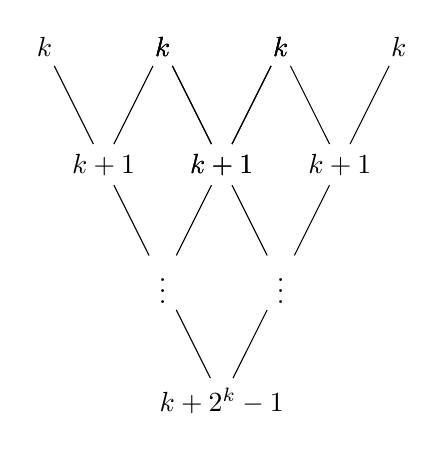
\begin{tikzpicture}[rotate=180]
\node {$k+2^k-1$}
    child {node {$\vdots$}
            child {node {$k+1$}
                child{node {$k$}}
                child{node {$k$}}
            }
            child {node {$k+1$}
                child{node {$k$}}
                child{node {$k$}}
            }
    }
    child{node {$\vdots$}
            child {node {$k+1$}
                child{node {$k$}}
                child{node {$k$}}
                }
            child {node {$k+1$}
                child{node {$k$}}
                child{node {$k$}}
                }
    };
\end{tikzpicture}

\end{document}